\documentclass[11pt, a4paper]{article}
\usepackage{pdfpages}
\usepackage{parallel}
\usepackage[T2A]{fontenc}
\usepackage{ucs}
\usepackage[utf8x]{inputenc}
\usepackage[polish,english,russian]{babel}
\usepackage{hyperref}
\usepackage{rotating}
\usepackage[inner=2cm,top=1.8cm,outer=2cm,bottom=2.3cm,nohead]{geometry}
\usepackage{listings}
\usepackage{graphicx}
\usepackage{wrapfig}
\usepackage{longtable}
\usepackage{indentfirst}
\usepackage{array}
\usepackage{tikzsymbols}
\usepackage{soul}
\usepackage[ruled,vlined]{algorithm2e}
%\counterwithout{figure}{section} 

\usepackage{url}
\makeatletter
\g@addto@macro{\UrlBreaks}{\UrlOrds}
\makeatother

\newcolumntype{P}[1]{>{\raggedright\arraybackslash}p{#1}}
\frenchspacing
\usepackage{fixltx2e} %text sub- and superscripts
\usepackage{icomma} % коскі ў матэматычным рэжыме
\PreloadUnicodePage{4}

\newcommand{\longpage}{\enlargethispage{\baselineskip}}
\newcommand{\shortpage}{\enlargethispage{-\baselineskip}}

\def\switchlang#1{\expandafter\csname switchlang#1\endcsname}
\def\switchlangbe{
\let\saverefname=\refname%
\def\refname{Літаратура}%
\def\figurename{Іл.}%
}
\def\switchlangen{
\let\saverefname=\refname%
\def\refname{References}%
\def\figurename{Fig.}%
}
\def\switchlangru{
\let\saverefname=\refname%
\let\savefigurename=\figurename%
\def\refname{Литература}%
\def\figurename{Рис.}%
}

\hyphenation{admi-ni-stra-tive}
\hyphenation{ex-pe-ri-ence}
\hyphenation{fle-xi-bi-li-ty}
\hyphenation{Py-thon}
\hyphenation{ma-the-ma-ti-cal}
\hyphenation{re-ported}
\hyphenation{imp-le-menta-tions}
\hyphenation{pro-vides}
\hyphenation{en-gi-neering}
\hyphenation{com-pa-ti-bi-li-ty}
\hyphenation{im-pos-sible}
\hyphenation{desk-top}
\hyphenation{elec-tro-nic}
\hyphenation{com-pa-ny}
\hyphenation{de-ve-lop-ment}
\hyphenation{de-ve-loping}
\hyphenation{de-ve-lop}
\hyphenation{da-ta-ba-se}
\hyphenation{plat-forms}
\hyphenation{or-ga-ni-za-tion}
\hyphenation{pro-gramming}
\hyphenation{in-stru-ments}
\hyphenation{Li-nux}
\hyphenation{sour-ce}
\hyphenation{en-vi-ron-ment}
\hyphenation{Te-le-pathy}
\hyphenation{Li-nux-ov-ka}
\hyphenation{Open-BSD}
\hyphenation{Free-BSD}
\hyphenation{men-ti-on-ed}
\hyphenation{app-li-ca-tion}

\def\progref!#1!{\texttt{#1}}
\renewcommand{\arraystretch}{2} %Іначай формулы ў матрыцы зліпаюцца з лініямі
\usepackage{array}

\def\interview #1 (#2), #3, #4, #5\par{

\section[#1, #3, #4]{#1 -- #3, #4}
\def\qname{LVEE}
\def\aname{#1}
\def\q ##1\par{{\noindent \bf \qname: ##1 }\par}
\def\a{{\noindent \bf \aname: } \def\qname{L}\def\aname{#2}}
}

\def\interview* #1 (#2), #3, #4, #5\par{

\section*{#1\\{\small\rm #3, #4. #5}}
\ifx\ParallelWhichBox\undefined%
    \addcontentsline{toc}{section}{#1, #3, #4}%
\else%
\ifnum\ParallelWhichBox=0%
    \addcontentsline{toc}{section}{#1, #3, #4}%
\fi\fi%

\def\qname{LVEE}
\def\aname{#1}
\def\q ##1\par{{\noindent \bf \qname: ##1 }\par}
\def\a{{\noindent \bf \aname: } \def\qname{L}\def\aname{#2}}
}

\newcommand{\interviewfooter}[1]{
\vskip 1em
\noindent \textit{#1}
}


\begin{document}

\title{1987 "--- IBM PS/2 mouse}
\date{}
\maketitle

В данной мыши, выпущенной в 1987 году, был впервые реализован интерфейс PS/2, до сих пор применяемый в ряде стационарных компьютеров подключения клавиатуры и мыши и использующий 6-контактный разъём mini-DIN.

\begin{figure}[h]
    \centering
    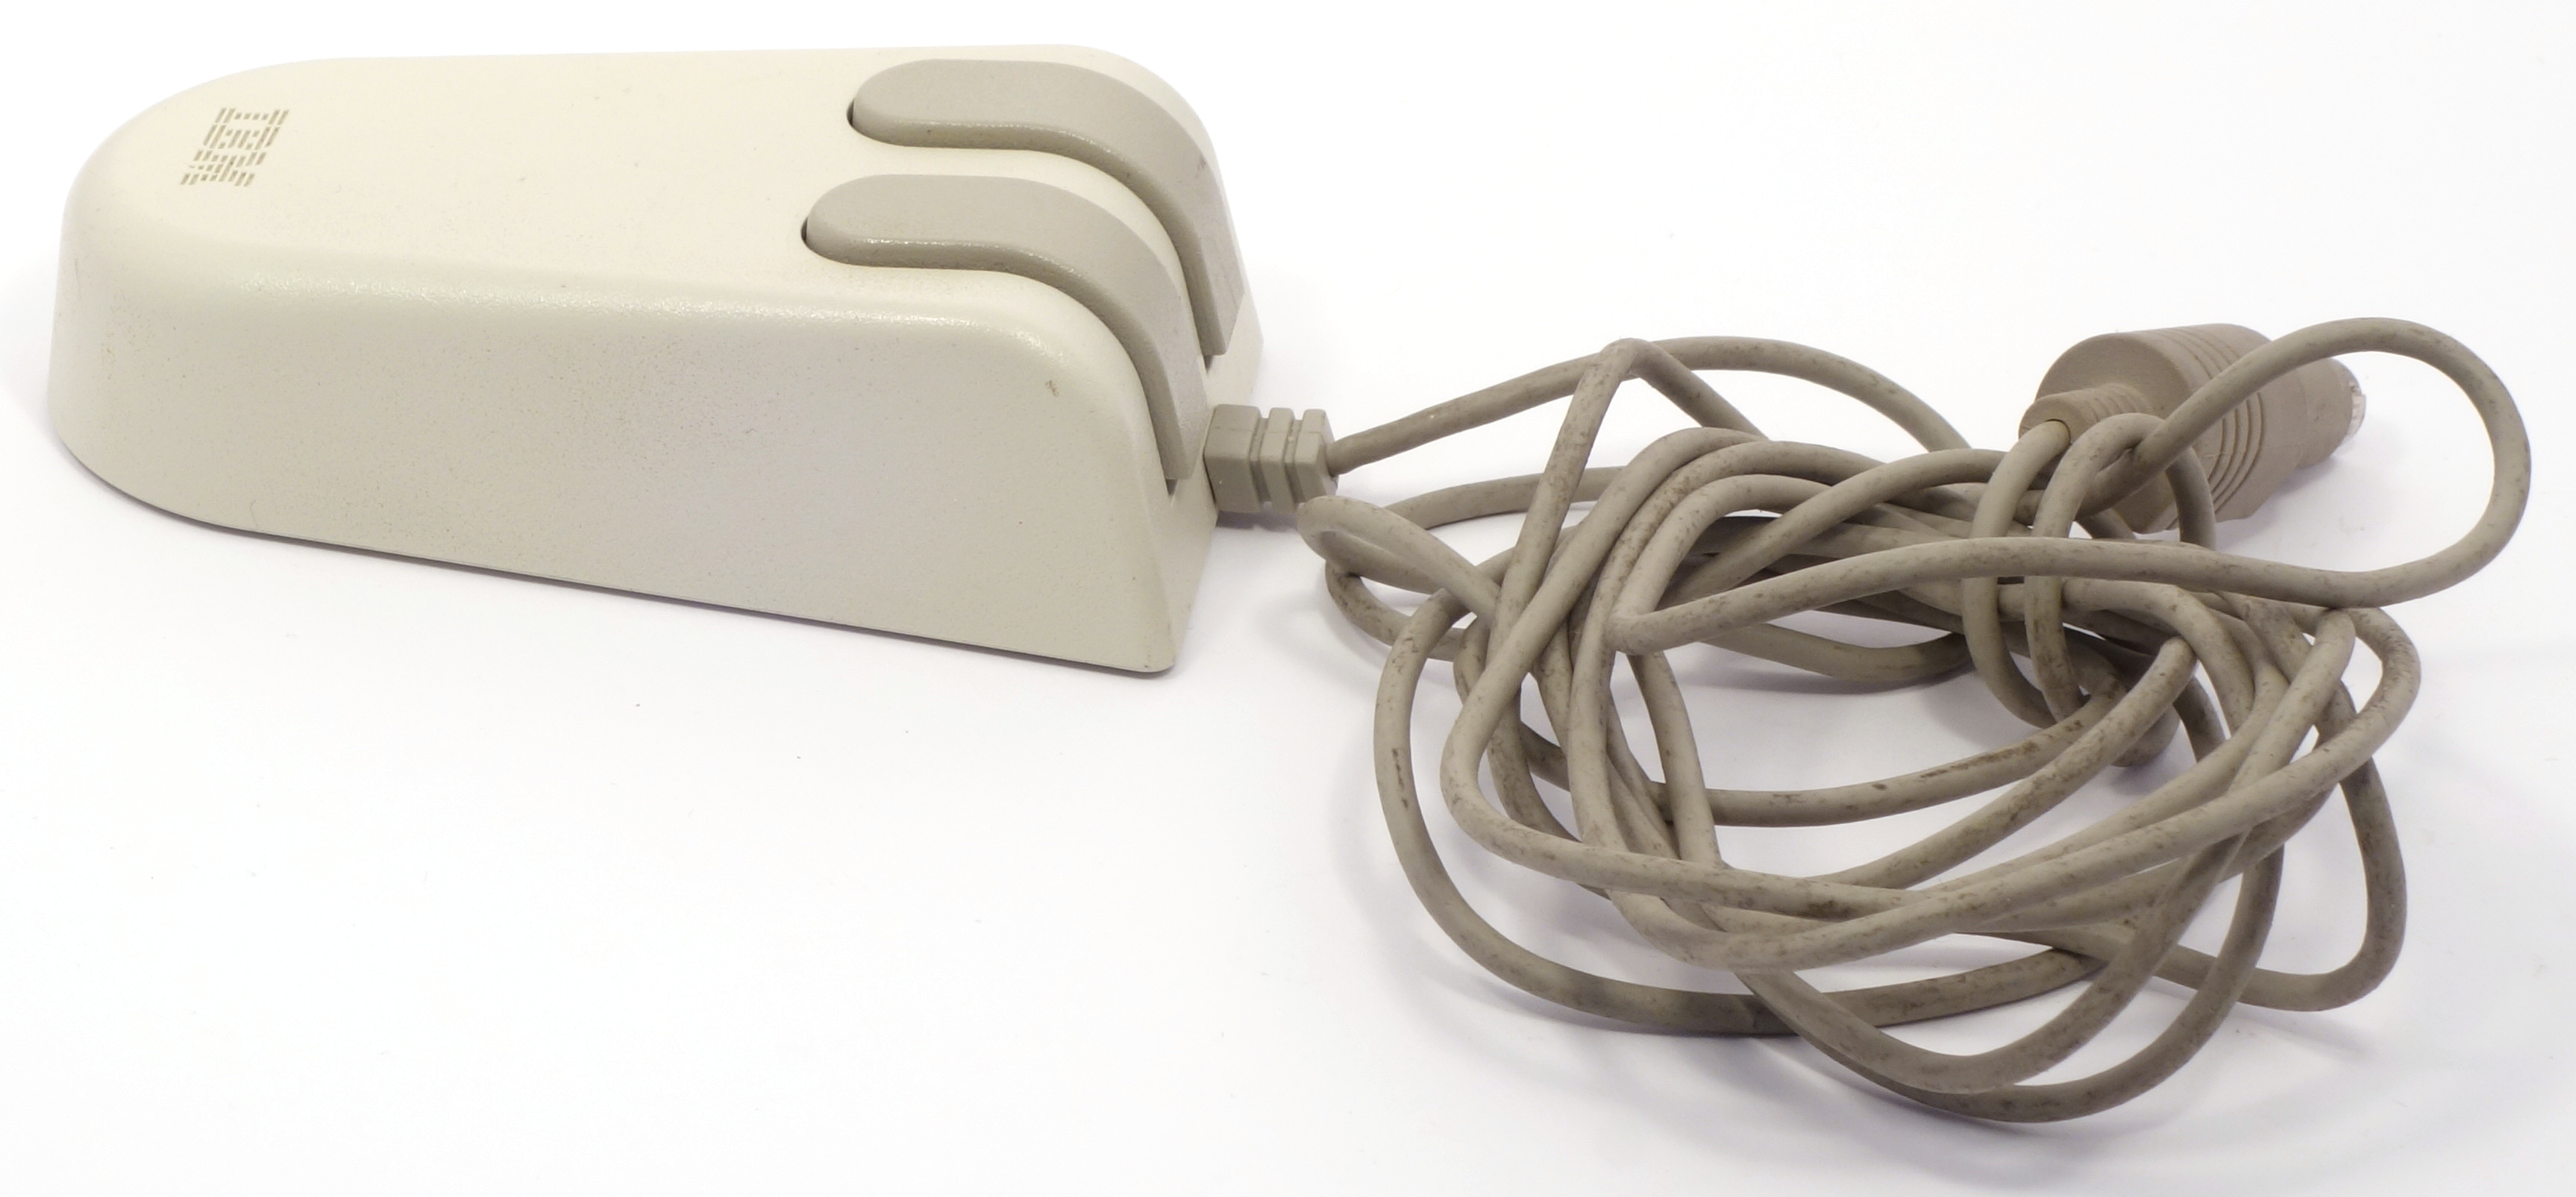
\includegraphics[width=\textwidth]{1987_ibm_ps2_mouse/num0.JPG}
    \caption{Мышь IBM PS/2 Mouse}
    \label{fig:IMBPS2Pic}
\end{figure}

Первой мышлью с этим интерфейсом, была доступная по сравнительно потребительским ценам в конце 80-х годов данная разработка компании IBM. Как можно видеть (рис. \ref{fig:IMBPS2TopBottom}), на верхней стороне корпуса присутствуют две механические кнопки для переключения и выгравирована эмблема компании; в целом корпус минималистичен и кроме этого не содержит никаких дополнительных элементов. Нижняя часть содержит шар, который хорошо скользит по поверхностям. Две стрелки на фиксаторе шара показывают, направление разблокировки, чтобы его можно было снять для чистки мыши.

\begin{figure}[h]
    \centering
    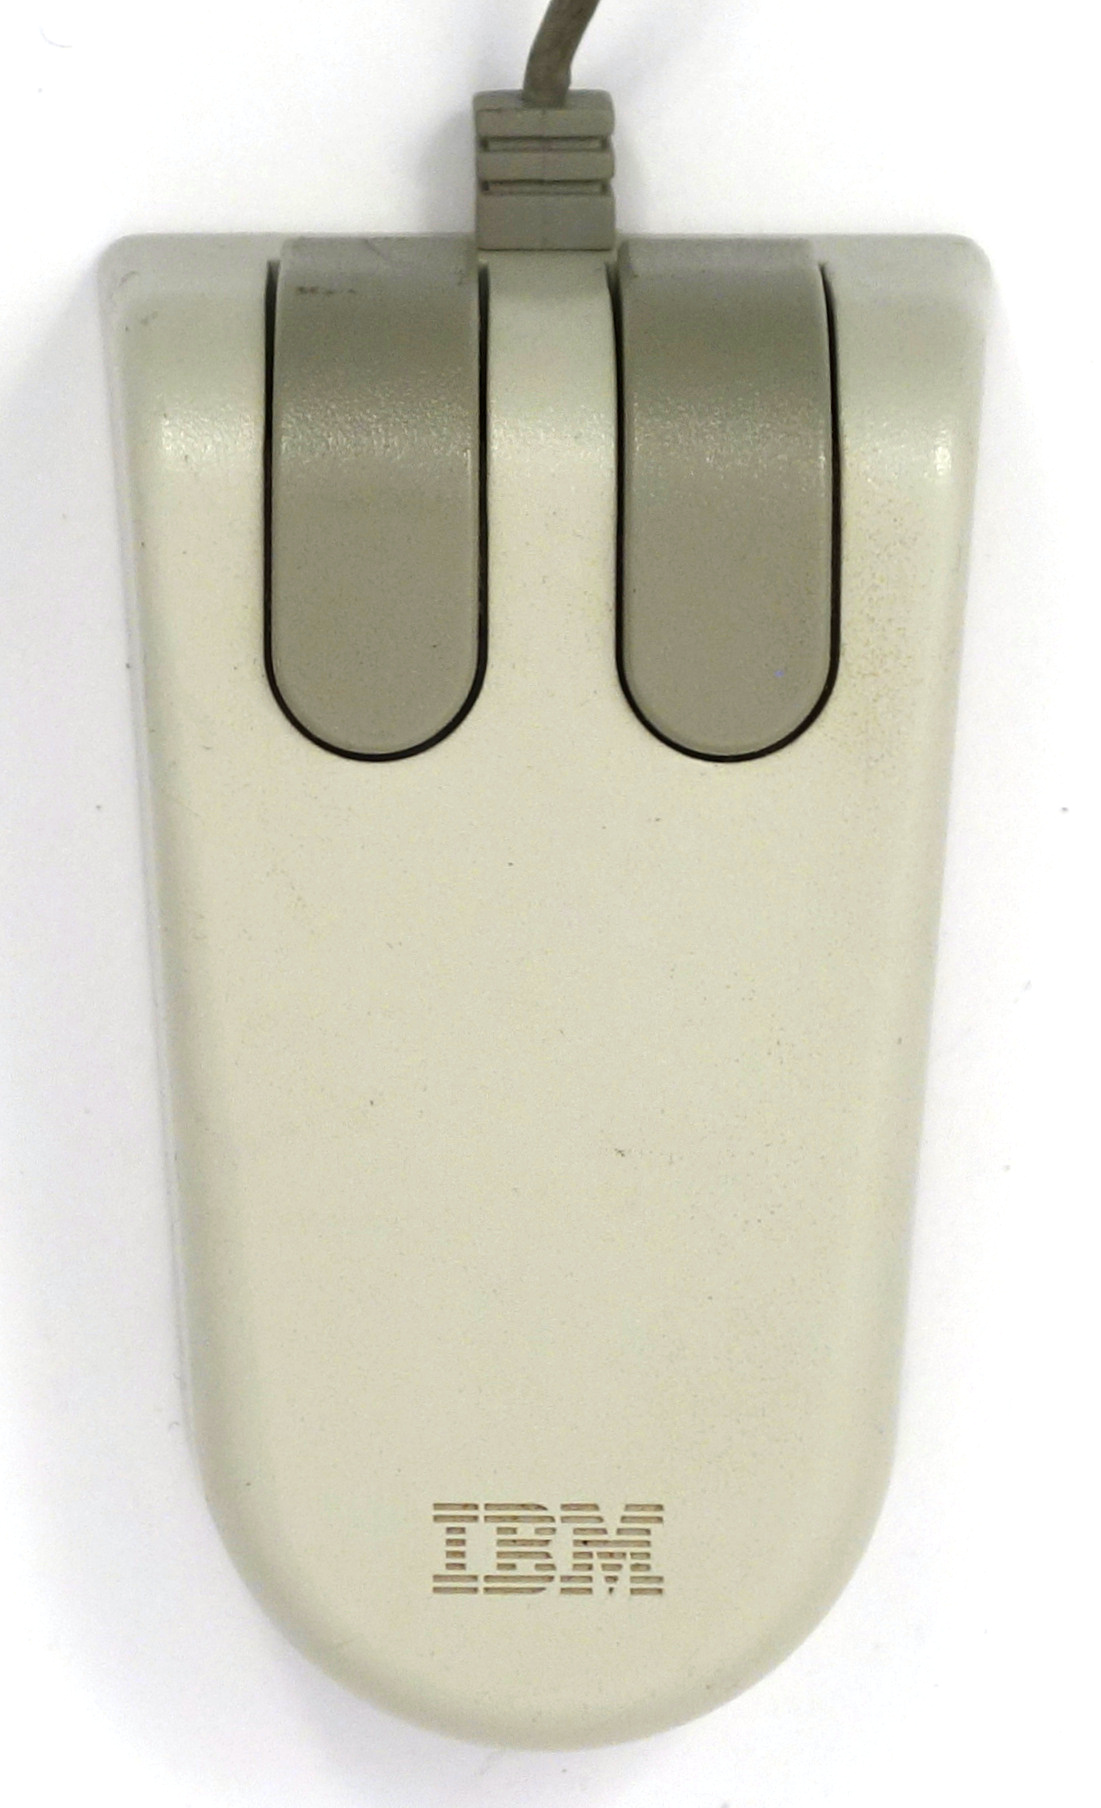
\includegraphics[scale=0.6]{1987_ibm_ps2_mouse/num1.JPG}
    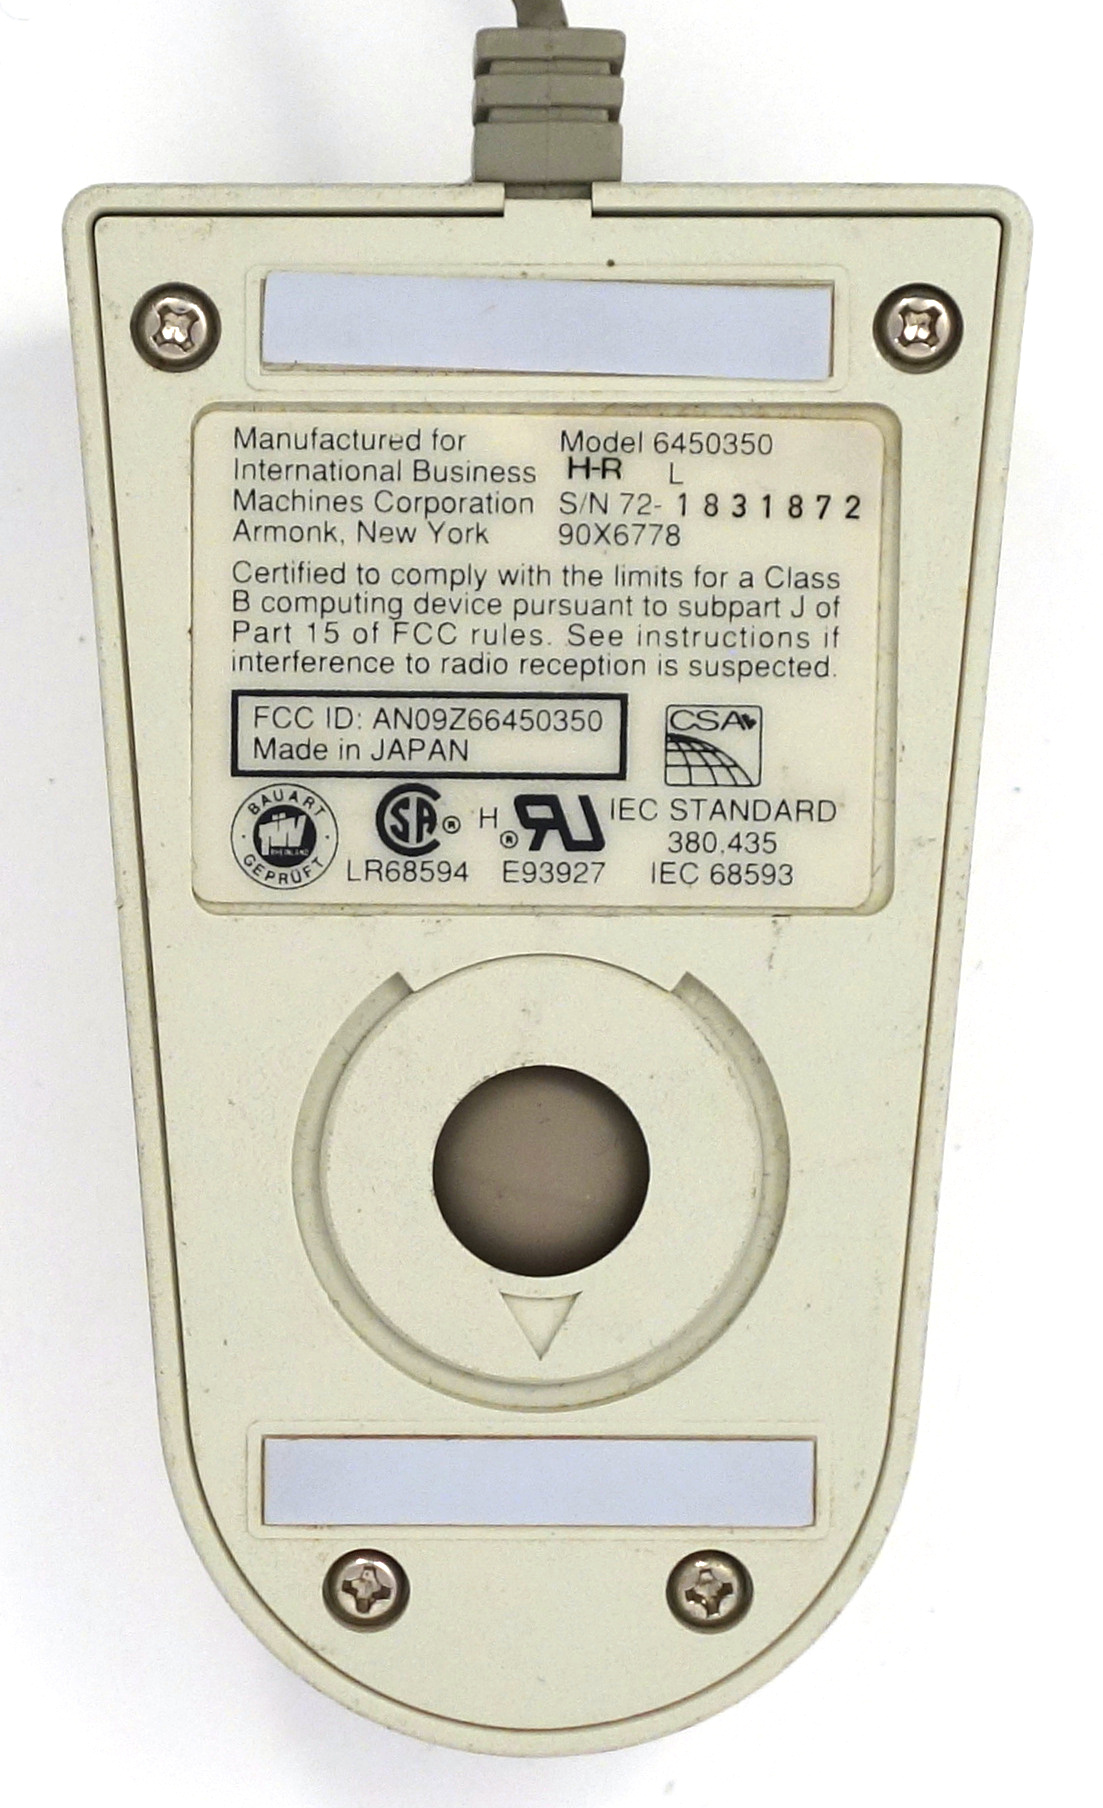
\includegraphics[scale=0.6]{1987_ibm_ps2_mouse/num2.JPG}
    \caption{IBM PS/2 Mouse, вид сверху и снизу}
    \label{fig:IMBPS2TopBottom}
\end{figure}

\begin{figure}[h]
    \centering
    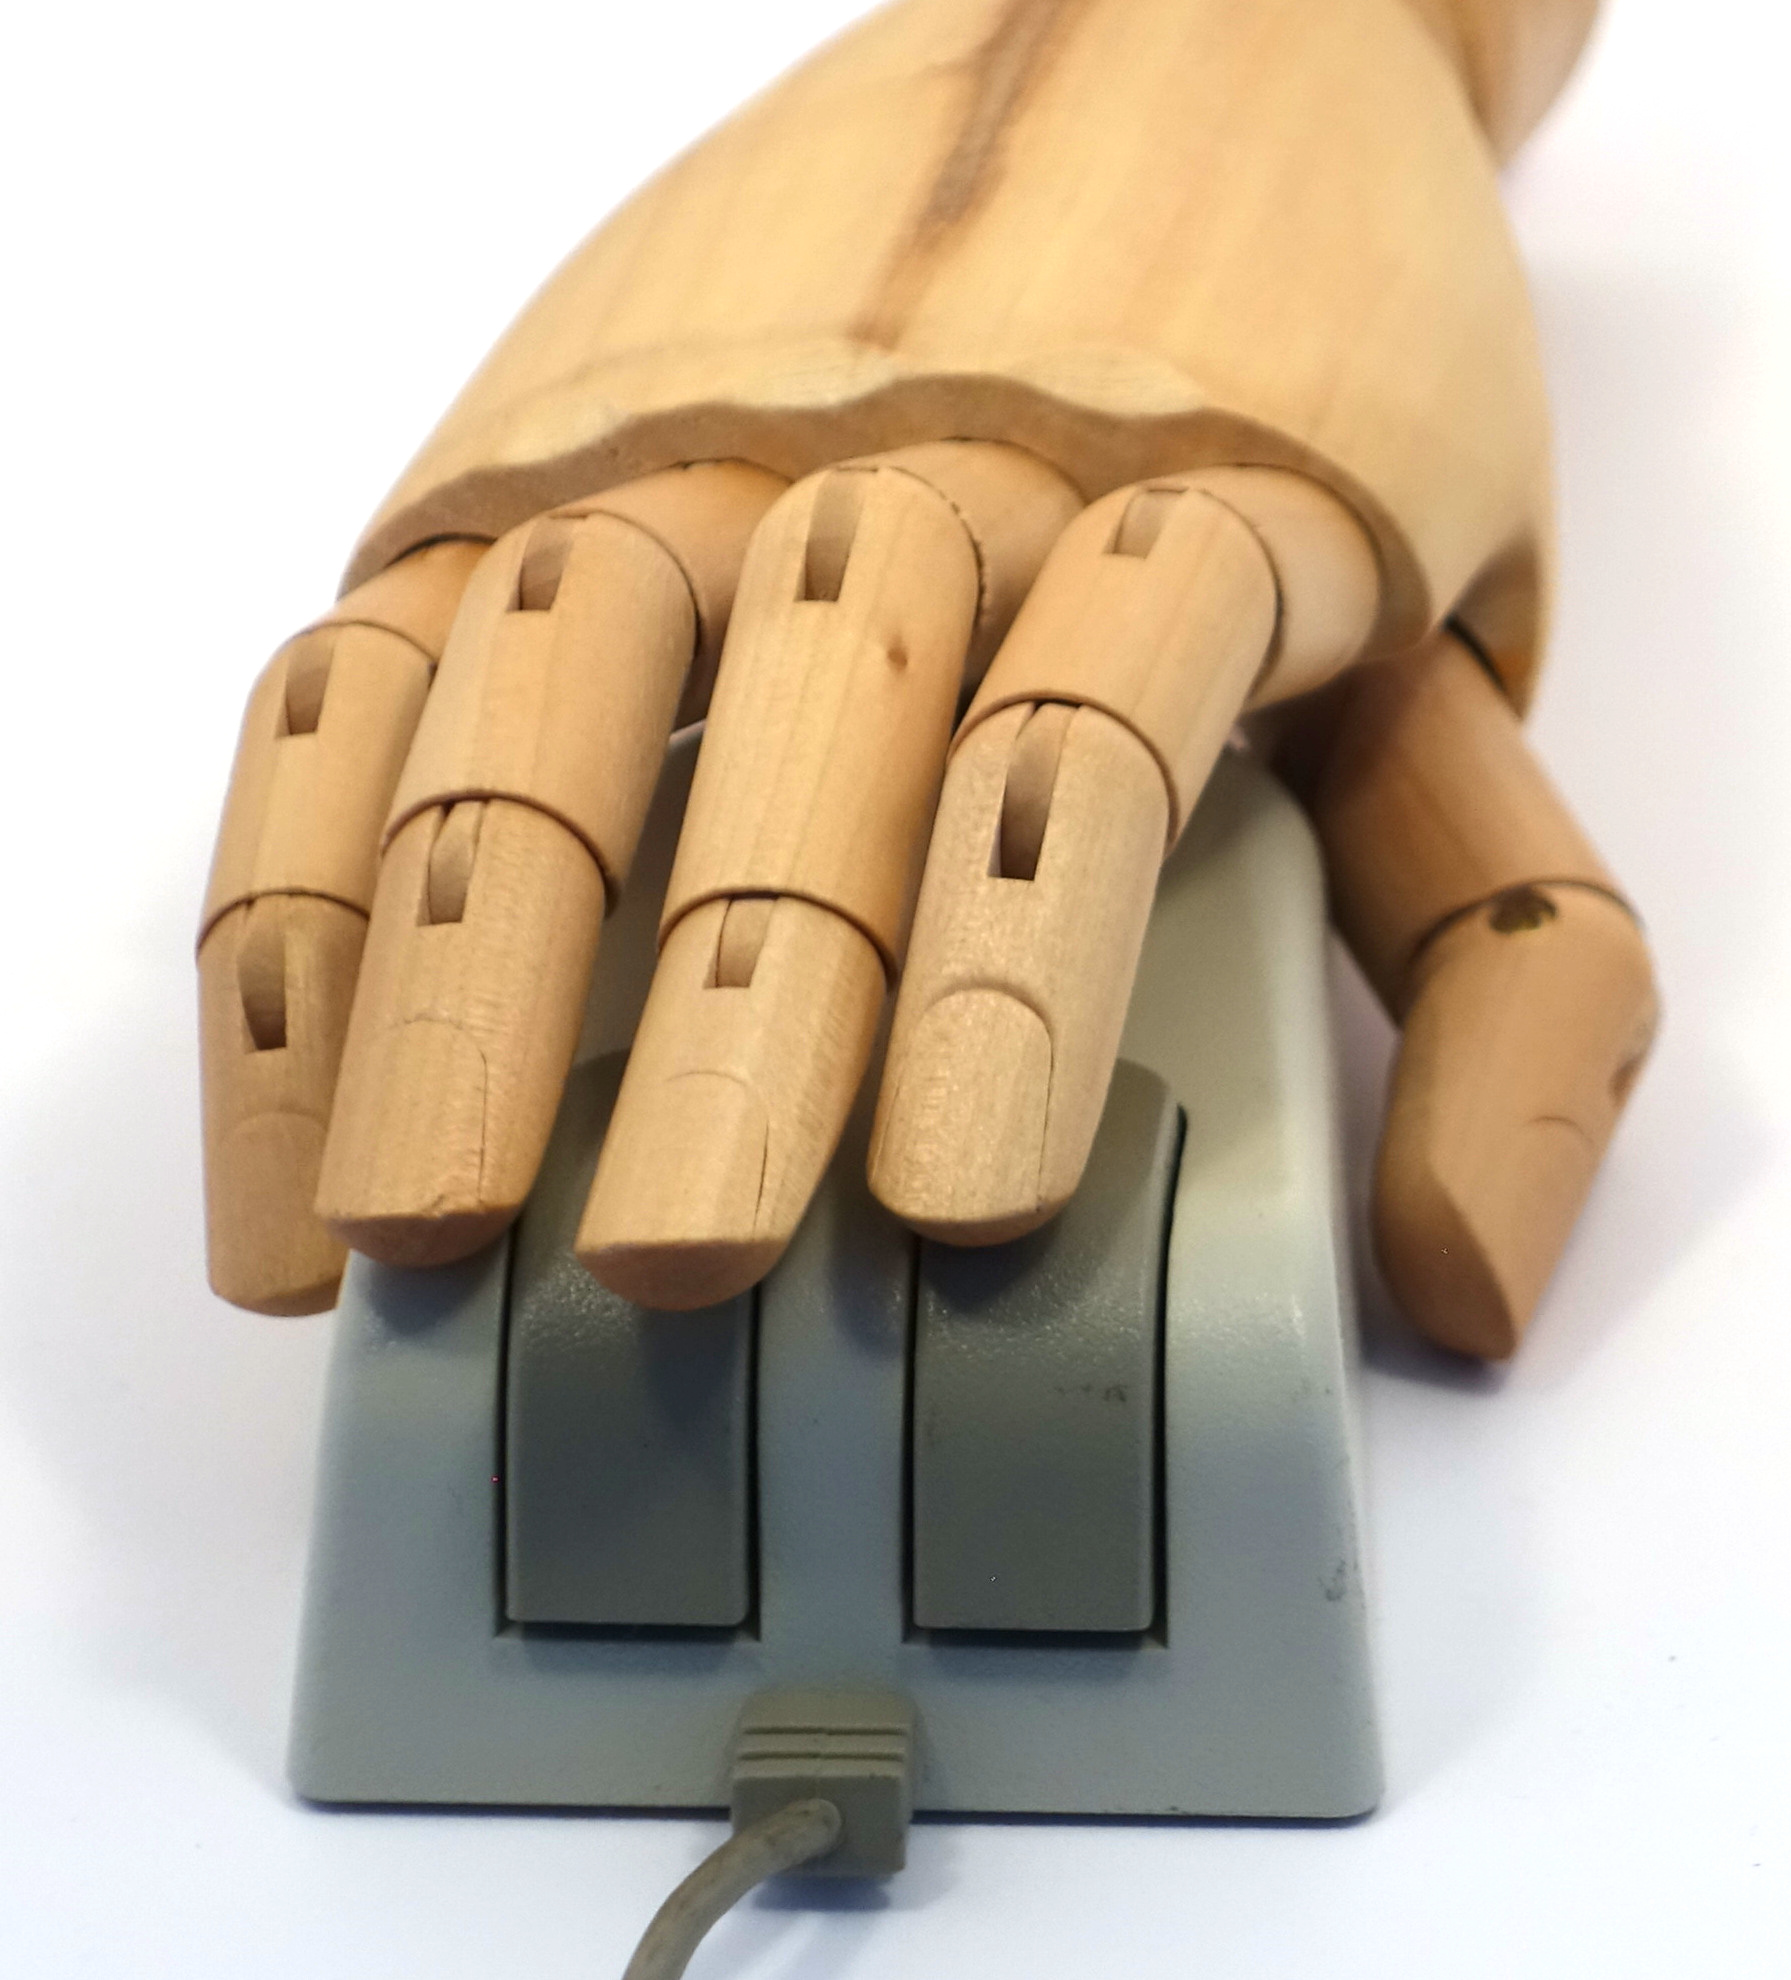
\includegraphics[scale=0.4]{1987_ibm_ps2_mouse/num3.JPG}
    \caption{Изображение IBM PS/2 Mouse с моделью руки человека}
    \label{fig:IMBPS2Hand}
\end{figure}

Как можно видеть на рис. \ref{fig:IMBPS2Hand}, трапециевидная форма корпуса позволяет достаточно комфортно обхватывать мышь пальцами, и нажимать кнопки при естественном положении кисти; однако маленькие размеры мыши (рис. \ref{fig:IMBPS2Size}) не позволяют опереться на ее корпус ладонью, что создает дополнительную нагрузку на запястье.

\begin{figure}[h]
    \centering
    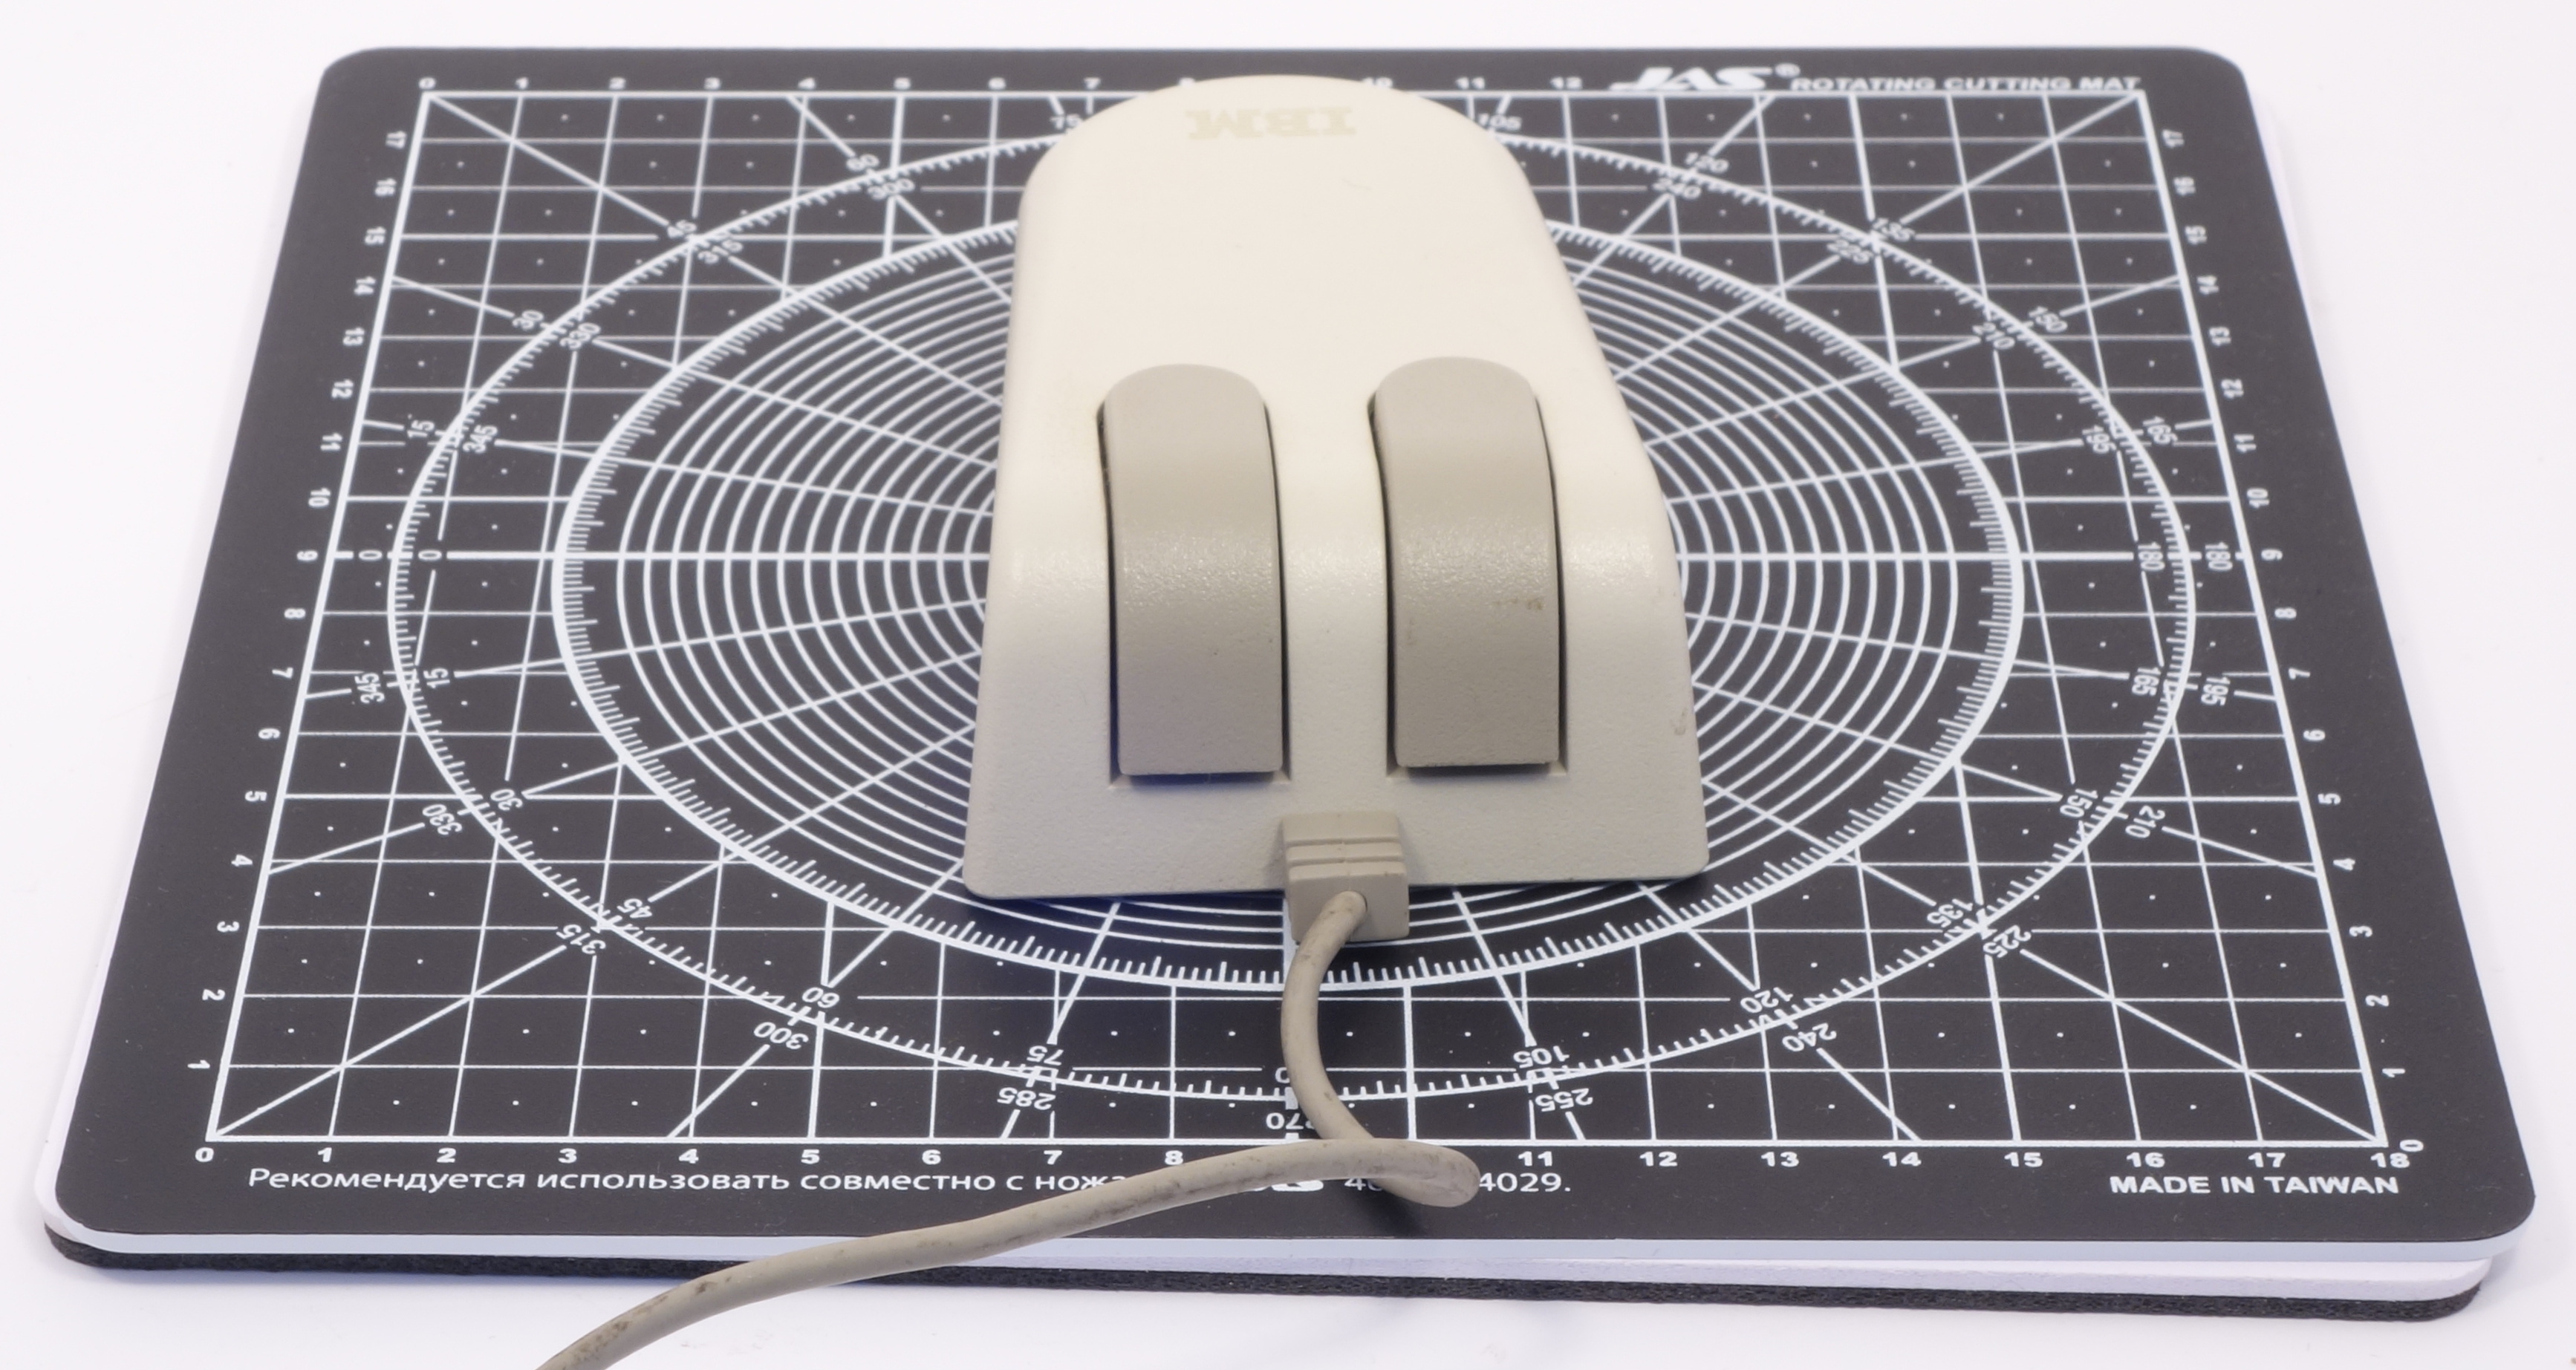
\includegraphics[scale=0.34]{1987_ibm_ps2_mouse/num4.jpg}
    \caption{Изображение IBM PS/2 Mouse на размерном коврике с шагом сетки 1~см}
    \label{fig:IBMPS2Size}
\end{figure}

\begin{figure}[h]
    \centering
    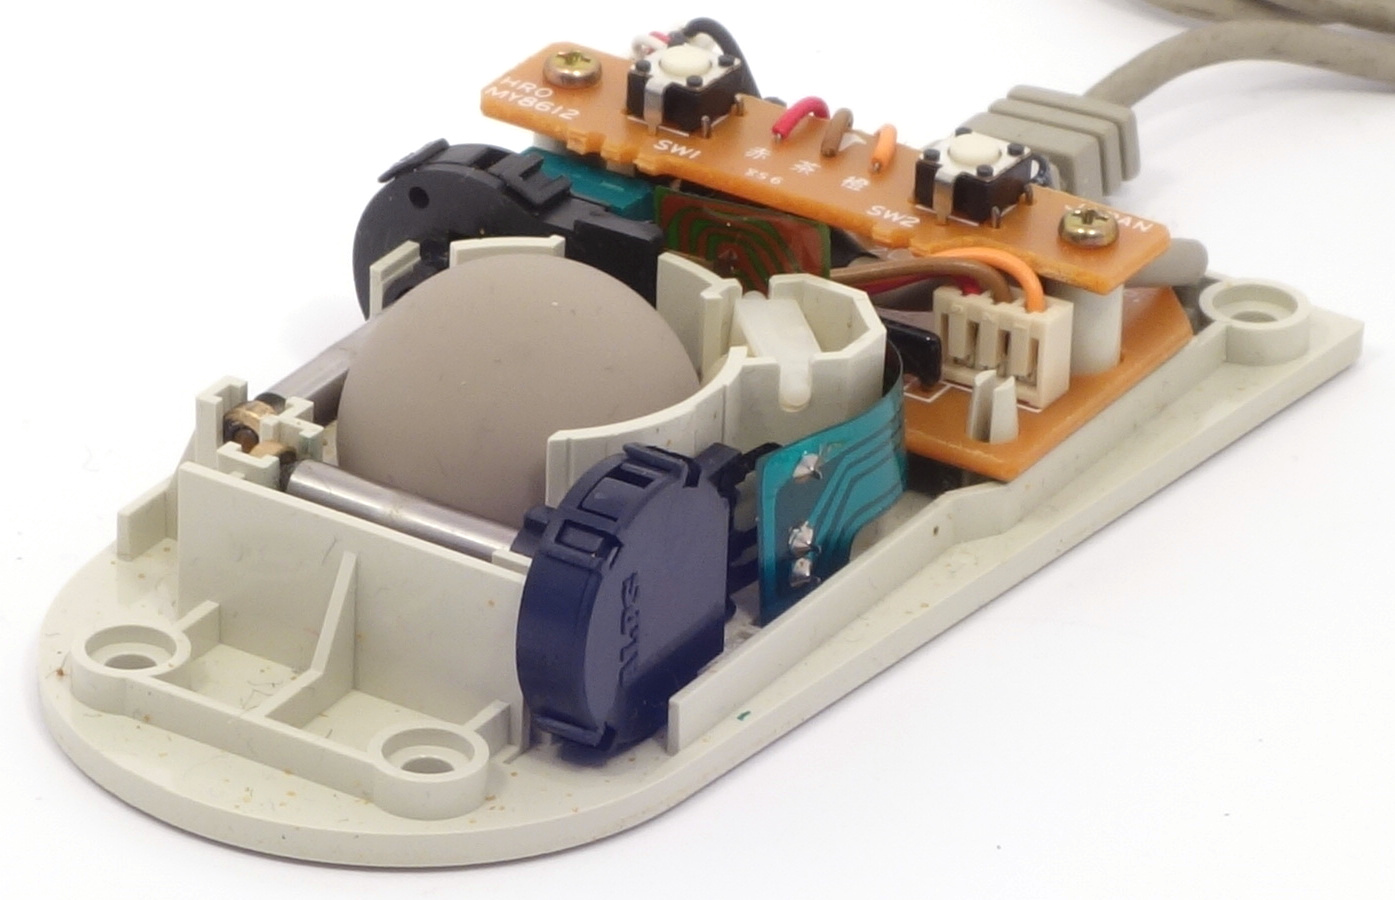
\includegraphics[scale=0.7]{1987_ibm_ps2_mouse/razob1.jpg} 
    \caption{IBM PS/2 Mouse в разобранном состоянии}
    \label{fig:IBMPS2Inside}
\end{figure}

Внутреннее устройство IBM PS/2 Mouse показано на рис. \ref{fig:IBMPS2Inside}, что позволяет классифицировать мышь как устройство с контактным энкодером, изготовленное в Японии компанией Alps. Необходимо отметить также массивные металлические ролики с подшипниками, характерные для дорогостоящих манипуляторов.
\end{document}
